% -*-latex-*-
\documentclass[dvips,handout]{beamer} 
%\documentclass[dvips,12pt]{beamer} 
\usepackage{etex,pictex}
\usepackage{color}
\title{The Dopamine D4 Story}
\author{Alan R. Rogers}
\date{\today}
\begin{document}

\frame{\titlepage}

\begin{frame}
\begin{columns}
\column{0.5\textwidth}
 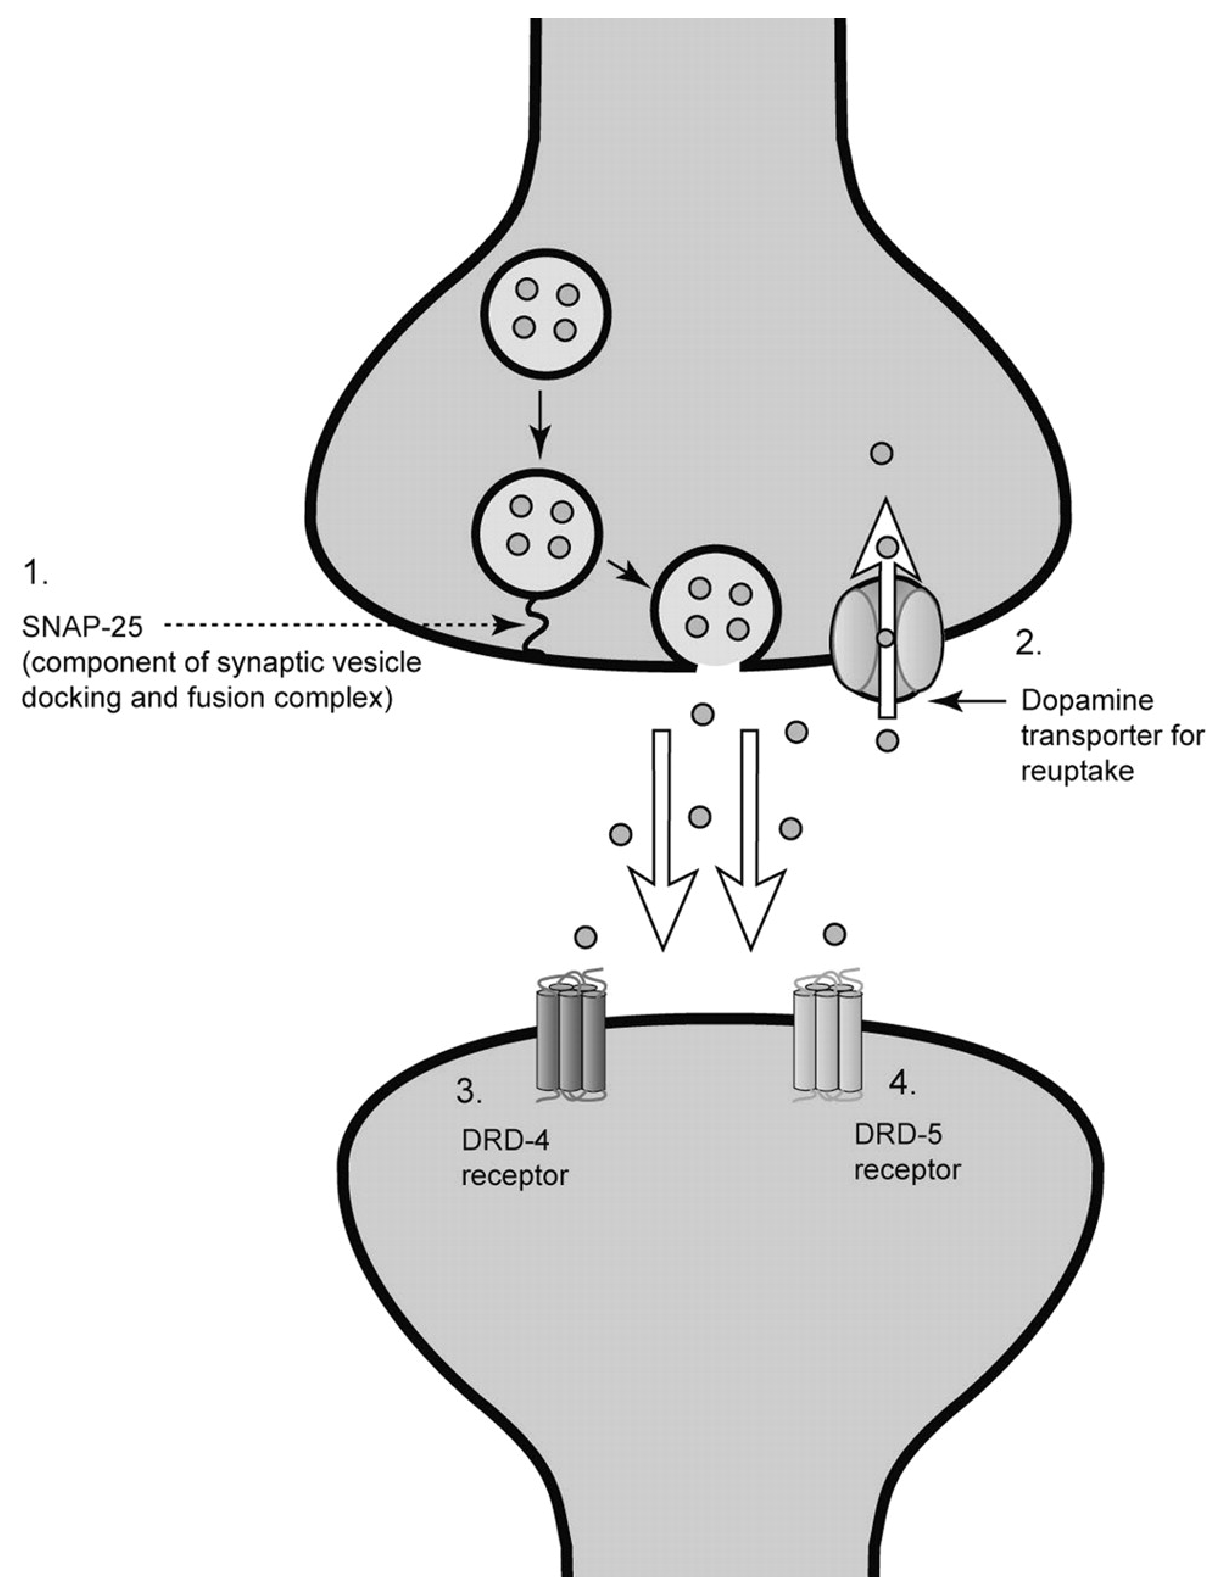
\includegraphics[width=\textwidth]{drd4synap.eps}
\column{0.5\textwidth}
\raggedright
\begin{itemize}
\item \emph{Neurons} are nerve cells
\item Communicate via molecules called \emph{neurotransmitters}
\item \emph{Dopamine} is one neurotransmitter
\item DRD4 is a type of dopamine receptor
\end{itemize}
\end{columns}
\end{frame}

\begin{frame}
\frametitle{Dopamine's effects (and associated problems)}
\begin{itemize}
\item control of movement (Parkinson's disease)
\item memory, attention, problem solving (ADHD)
\item mood (depression)
\item pleasure and motivation (addiction)
\item sociability (social anxiety)
\end{itemize}
\end{frame}

\begin{frame}
\frametitle{The D4 dopamine receptor (DRD4) gene}
\begin{itemize}
\item One of 5 receptors
\item Lots of variation within human populations
\item Several alleles: 4R (common), 7R (less common), etc
\end{itemize}
\end{frame}

\begin{frame}
\frametitle{Attention Deficit Hyperactivity
      Disorder (ADHD)}
\begin{itemize}
\item Children with ADHD have trouble sitting still and paying attention.
\item Primarily in boys.
\item Affects 3--5\% of children.
\end{itemize}
\end{frame}

\begin{frame}
\frametitle{Association between DRD4-7R and ADHD}
\begin{itemize}
\item Some ADHD children do not carry the 7R allele.
\item Some 7R carriers do not have ADHD.
\item But among 7R carriers, the frequency of ADHD is 
twice as high.
\item Does 7R reduce Darwinian fitness?
\end{itemize}
\end{frame}

\begin{frame}
Harmful alleles are always
\begin{enumerate}
\item rare, and
\item new.
\end{enumerate}
Rare because selection keeps them rare, and new because selection
doesn't let them last long.

Is this true of the 7R allele?
\end{frame}

\begin{frame}
\frametitle{Frequencies of DRD4 alleles}
\begin{center}
\begin{tabular}{lr}
2R &  8.8\%\\
4R & 65.1\%\\
7R & 19.2\%\\
others & 6.9\%
\end{tabular}\\

\bigskip

The 7R allele is \emph{NOT} rare.  Is it new?
\end{center}
\end{frame}

\begin{frame}[containsverbatim]
\frametitle{Relationships among DRD4 alleles}
\begin{verbatim}
       2R <-- 4R --> --> --> --> 7R

           1           4-5
        mutation    mutations
\end{verbatim}
\begin{itemize}
\item 4R is ancestral
\item 2R and 7R are derived
\item many mutational steps separate 4R and 7R.
\item 7R is \emph{NOT} new.
\end{itemize}
\end{frame}

\begin{frame}
\frametitle{Puzzle}
The 7R allele causes a harmful condition,
yet it is neither new nor rare.

What gives?

Let us look for evidence of selection.
\end{frame}

\begin{frame}
\begin{columns}
\column{0.6\textwidth}
 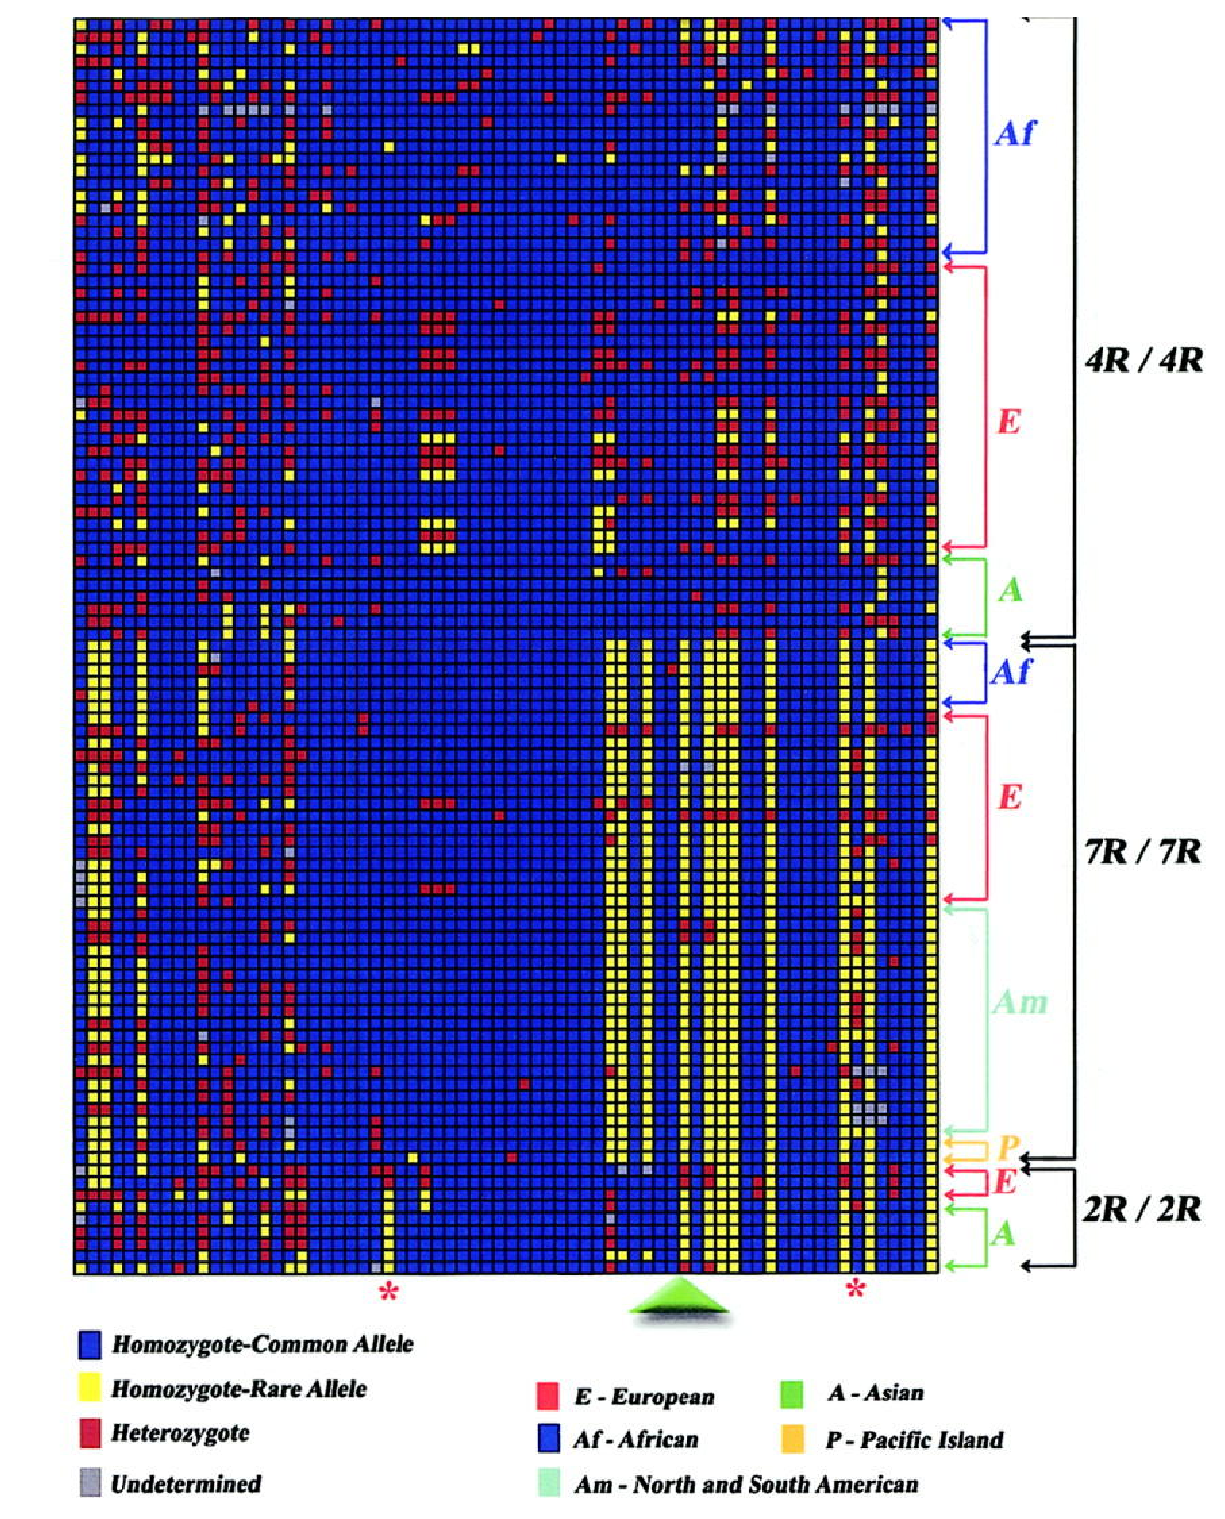
\includegraphics[width=\textwidth]{drd4-polymorph.eps}
\column{0.4\textwidth}
\raggedright
\begin{itemize}
\item Columns are SNPs
\item Rows are diploid genotypes
\item Blue: common homozygote
\item Yellow: rare homozygote
\item Red: heterozygote
\item Note LD w/i 7R genotypes
\end{itemize}
\end{columns}
\end{frame}

\begin{frame}
\frametitle{Fraction of Recombinant Chromosomes (FRC))}
 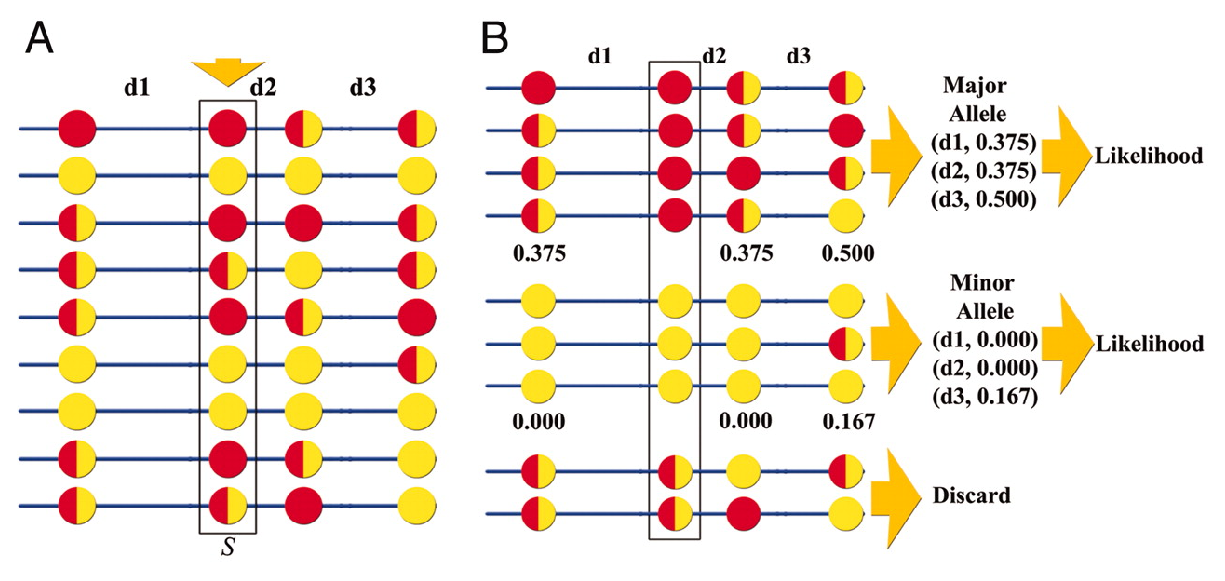
\includegraphics[width=\textwidth]{wang-frc.eps}
\end{frame}

\begin{frame}
\begin{columns}
\column{0.8\textwidth}
 \includegraphics[width=\textwidth]{drd4-ld.eps}
\column{0.3\textwidth}
\raggedright
\begin{itemize}
\item Few recombinants near selected site
\item on 7R allele.
\item Shows allele is young.
\end{itemize}
\end{columns}
\end{frame}

\begin{frame}
\begin{itemize}
\item 7R is young but not rare.
\item Must have increased in frequency rapidly.
\item Has been favored by selection.
\end{itemize}
\end{frame}

\begin{frame}
\frametitle{When did this selection start?}
The number of recombinants implies that it started about 40~kyr ago.

Roughly the time of the expansion of modern humans.
\end{frame}

\begin{frame}
\frametitle{The puzzle again}
How can the 7R allele be favored by selection if it
causes a disease?

Either
\begin{itemize}
\item it has some compensating advantage, or
\item ADHD is only a problem in today's environment.
\end{itemize}
\end{frame}

\begin{frame}
\frametitle{7R carriers tend to have several other characteristics}
\begin{itemize}
\item novelty seeking
\item perseverance
\item fast reaction times
\item sexuality
\end{itemize}
These may be fitness enhancing, at least in some situations.
\end{frame}

\begin{frame}
\begin{columns}
\column{0.7\textwidth}
\includegraphics[width=\textwidth]{drd4-macmig.eps}
\column{0.3\textwidth}
\raggedright
Long (mainly 7R) alleles are common in groups far from origin of their
language families.  
\end{columns}
\end{frame}

\begin{frame}
\begin{itemize}
\item
7R is common in groups that have moved far from the origin of their
     language family.
Populations
\item
Also more common in nomadic groups than in sedentary ones.
\end{itemize}
\end{frame}

\begin{frame}
\frametitle{Distribution of DRD4 alleles}
 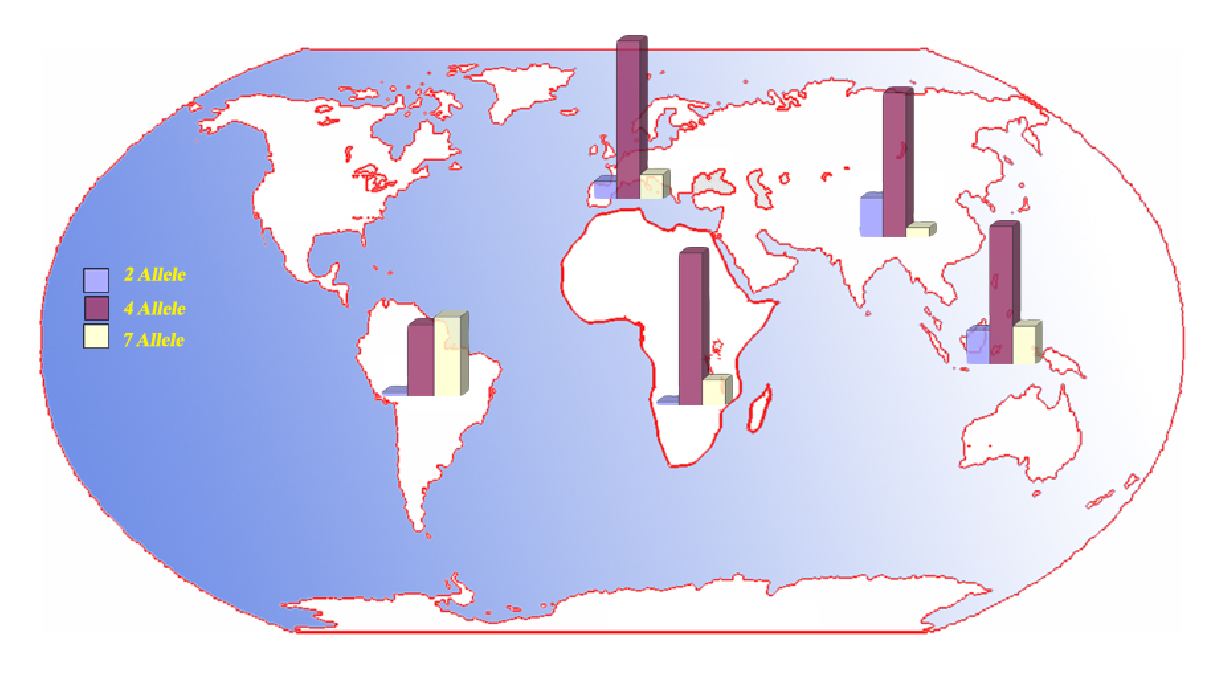
\includegraphics[width=\textwidth]{drd4map.eps}
\end{frame}

\begin{frame}
7R most common far from Africa---except for China\\
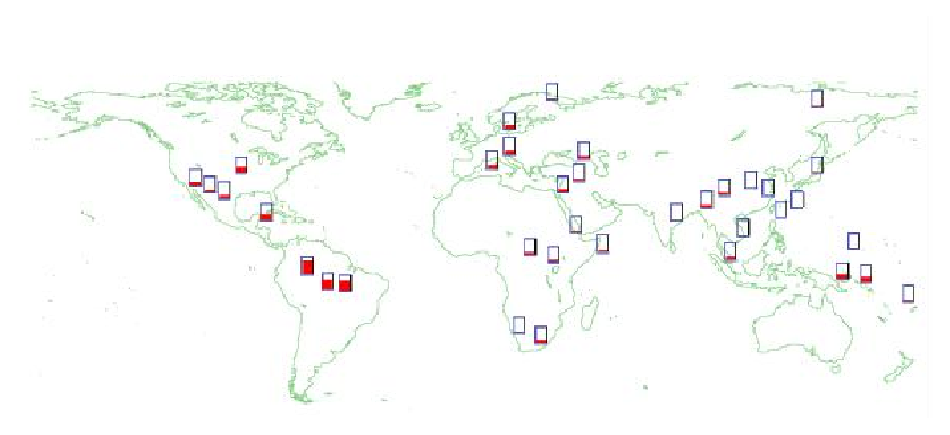
\includegraphics[width=\textwidth]{drd4-7rmap.eps}
\end{frame}

\begin{frame}
\frametitle{Hypothesis of Ding et al (2002)}
\begin{itemize}
\item 7R allele predisposes carriers to novelty seeking and
      perseverance. 
\item More likely to move.
\item Each generation, 7R allele more common among migrants.
\item Frequency increases with distance from Africa.
\item Works for Oceania and South America
\item What about China
\end{itemize}
\end{frame}

\begin{frame}
\frametitle{7R was probably once in China}
Although 7R is absent there, China does contain alleles derived from
7R.
\end{frame}

\begin{frame}
\frametitle{Summary}
\begin{itemize}
\item DRD4 Dopamine receptor is highly variable
\item and affects behavior in various ways.
\item The 7R allele predisposes its bearers to
ADHD.
\item Harmful alleles are usually rare and new, but 7R is neither.
\item Has been favored by selection for 40~kyr.
\item Hypothesis of Ding et al.
\begin{itemize}
\item 7R allele predisposes carriers to novelty-seeking
\item and to mobility.
\item Most common in populations far from Africa.
\end{itemize}
\end{itemize}
\end{frame}

\end{document}